%!TEX root = ../template.tex
%%%%%%%%%%%%%%%%%%%%%%%%%%%%%%%%%%%%%%%%%%%%%%%%%%%%%%%%%%%%%%%%%%%
%% chapter1.tex
%% NOVA thesis document file
%%
%% Chapter with introduction
%%%%%%%%%%%%%%%%%%%%%%%%%%%%%%%%%%%%%%%%%%%%%%%%%%%%%%%%%%%%%%%%%%%

\typeout{NT FILE 03_statement.tex}%

\chapter{Research Statement}\label{cha:statement}

% The Research Statement should explain the intended research work, including a
% description of the kind of issues and problem(s) to address, their motivation,
% the vision and ideas on how they may be tackled, their novelty, and the
% expected results. This presentation should be cohesively cross-referenced to
% the survey included in the previous chapter.

% ------------------------------------
\section{Power Grid Inspections Powered by 3D Vision}\label{sec:ts40k}

\begin{figure}[ht]
      \centering
      % First column: Full width figure and subfigures
      \begin{minipage}[t]{0.51\textwidth} % First column
            \begin{subfigure}[b]{\textwidth}
                  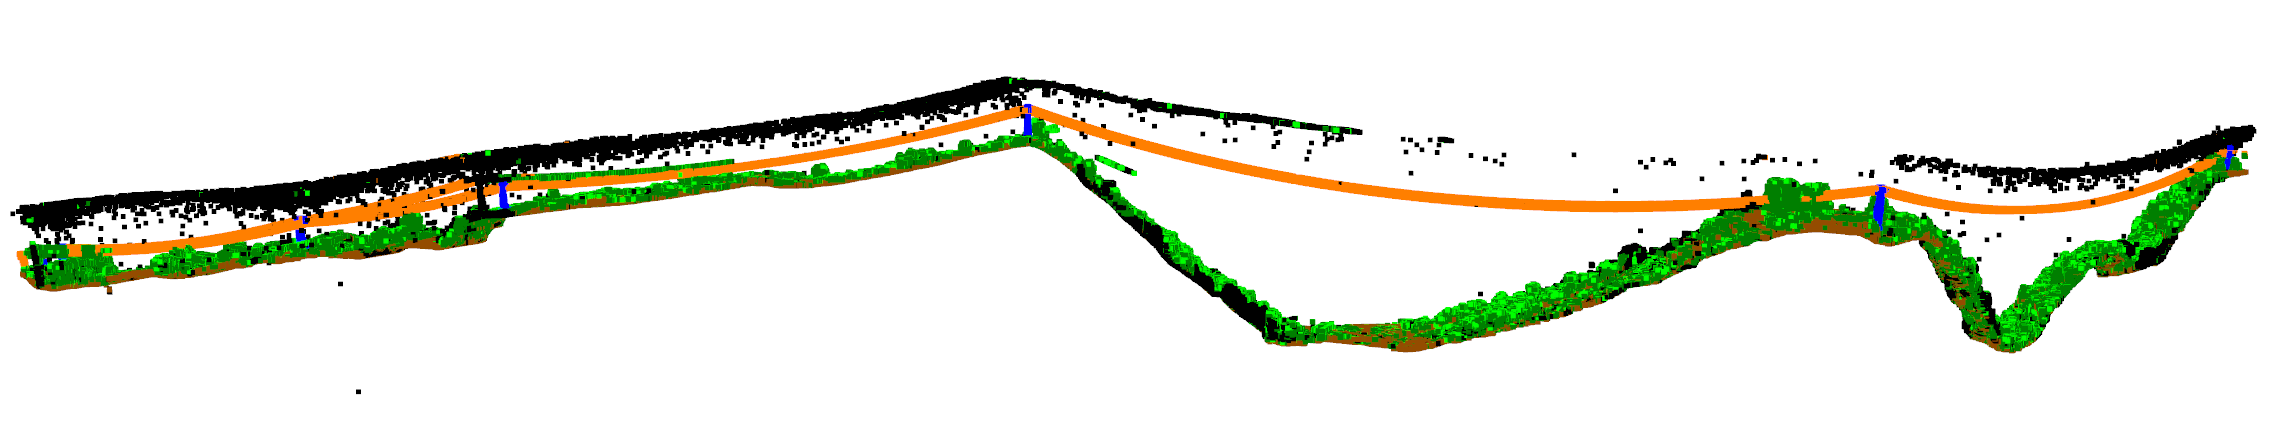
\includegraphics[width=\linewidth]{ts40k/Teaser/raw_sample.png}
                  \caption{Raw TS40K sample}
                  \label{fig:teaser-raw-sample}
            \end{subfigure}
            \vfill
            \begin{subfigure}[b]{0.33\textwidth}
                  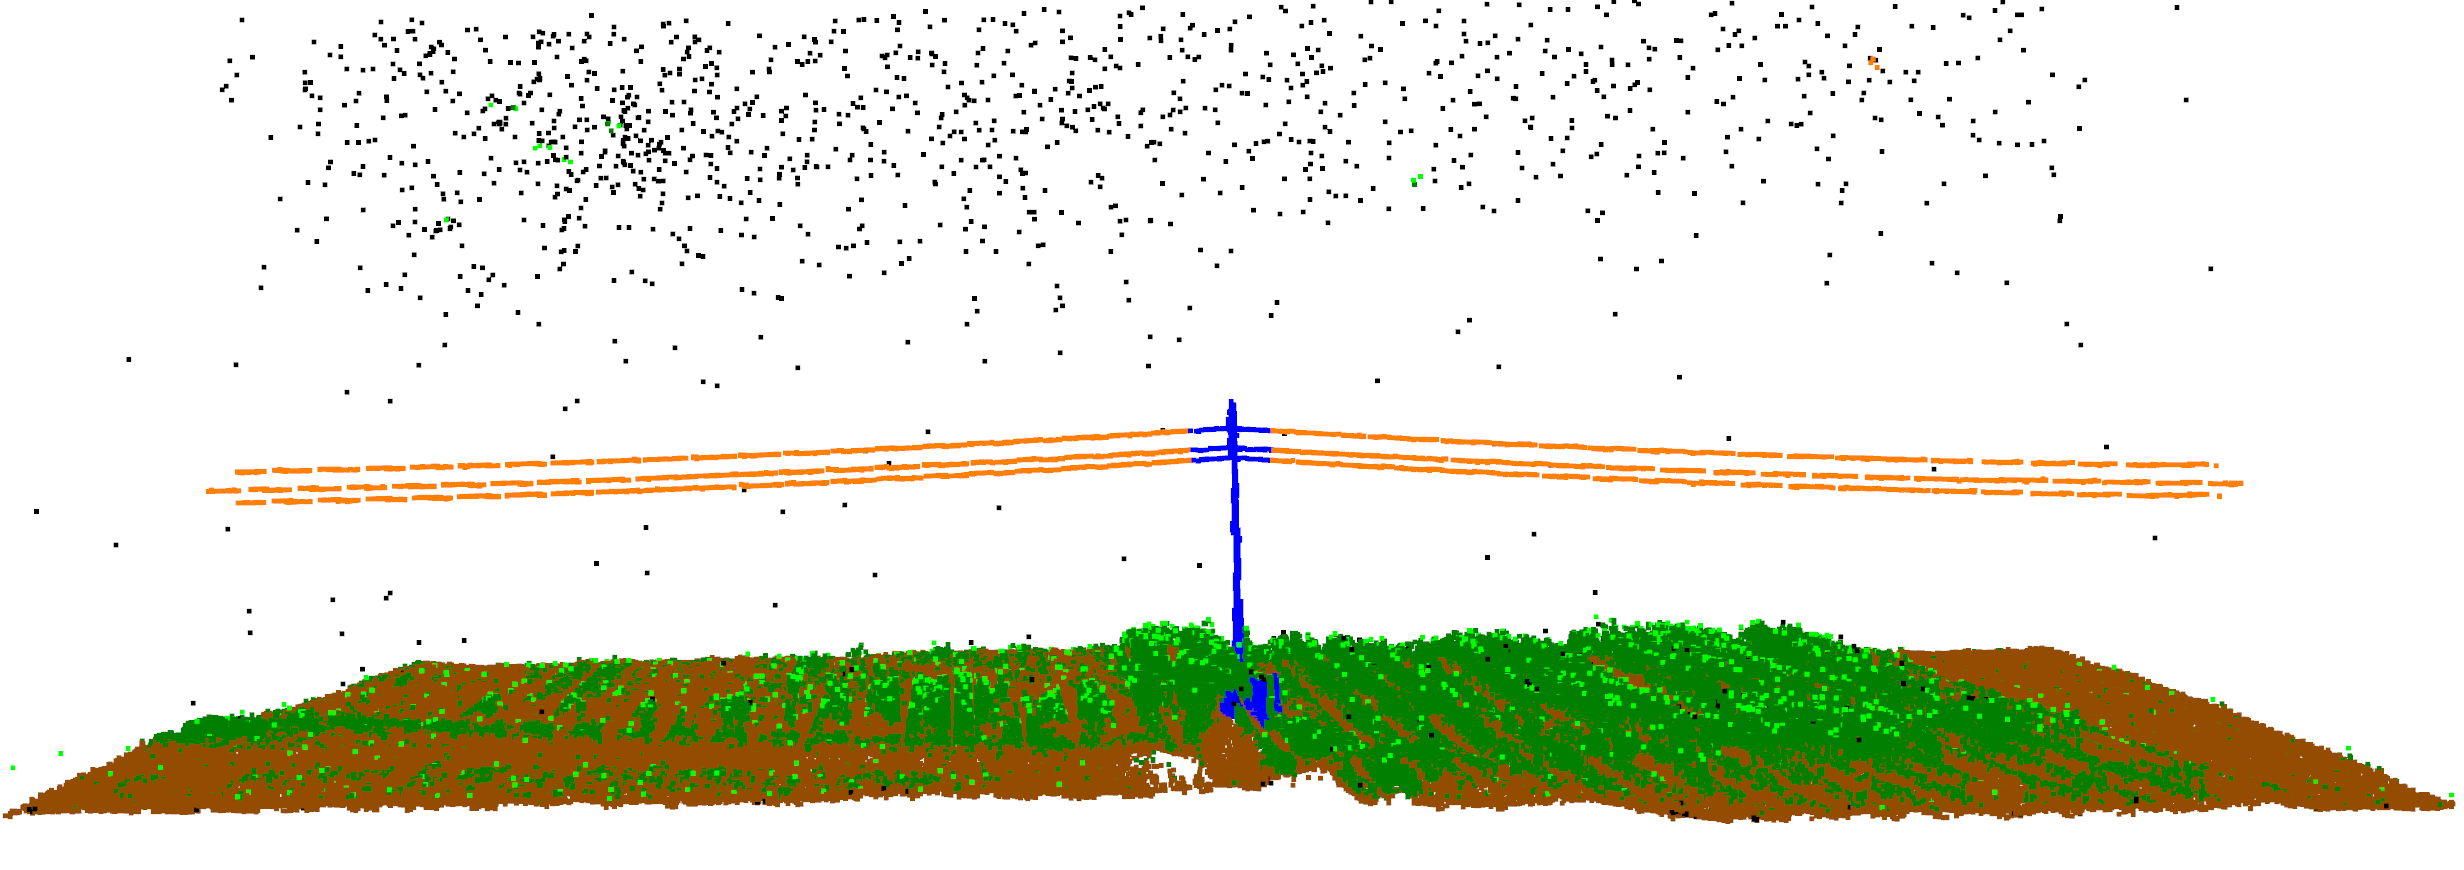
\includegraphics[width=\linewidth]{ts40k/Teaser/tower_radius.png}
                  \caption{Tower-radius}
                  \label{fig:teaser-tower-radius}
            \end{subfigure}
            \hfill
            \begin{subfigure}[b]{0.33\textwidth}
                  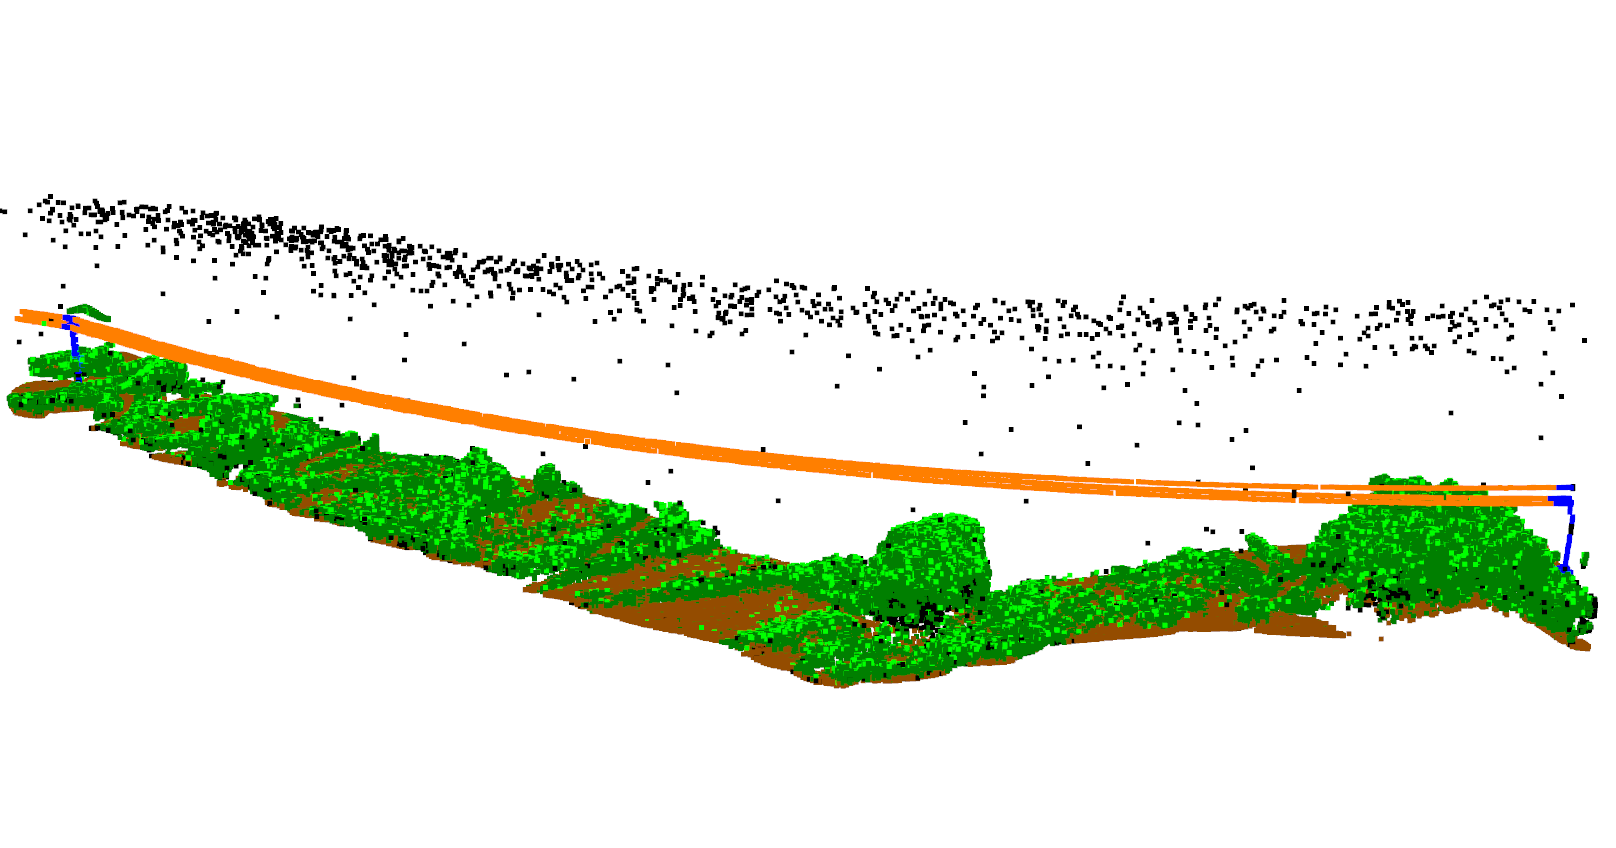
\includegraphics[width=\linewidth]{ts40k/Teaser/2_towers.png}
                  \caption{Power-line}
                  \label{fig:teaser-power-line}
            \end{subfigure}
            \hfill
            \begin{subfigure}[b]{0.30\textwidth}
                  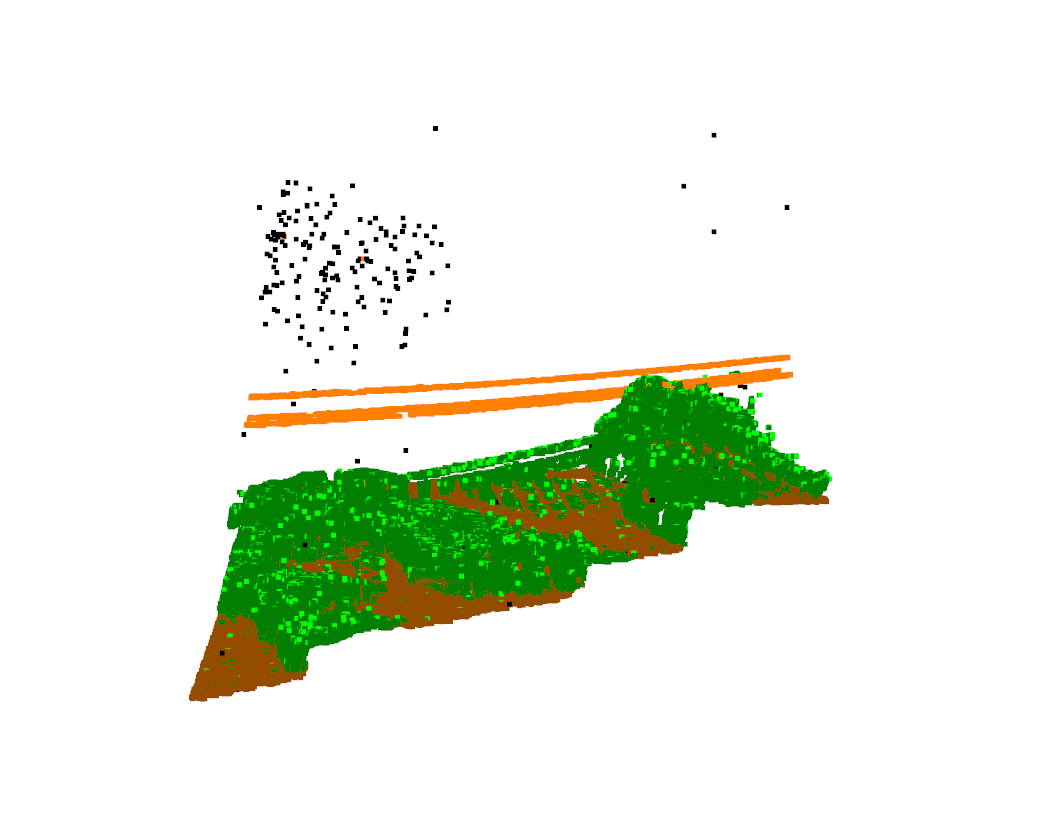
\includegraphics[width=\linewidth]{ts40k/Teaser/no_ts.png}
                  \caption{No-tower}
                  \label{fig:teaser-no-ts}
            \end{subfigure}
            \vfill
            % Legend below subfigures
            
\includegraphics[width=\linewidth]{ts40k/legend_classes.png}
      \end{minipage}
      \quad
      % Second column: Two additional figures
      \begin{minipage}[t]{0.45\textwidth} % Second column
            \begin{subfigure}[b]{1.0\textwidth}
                  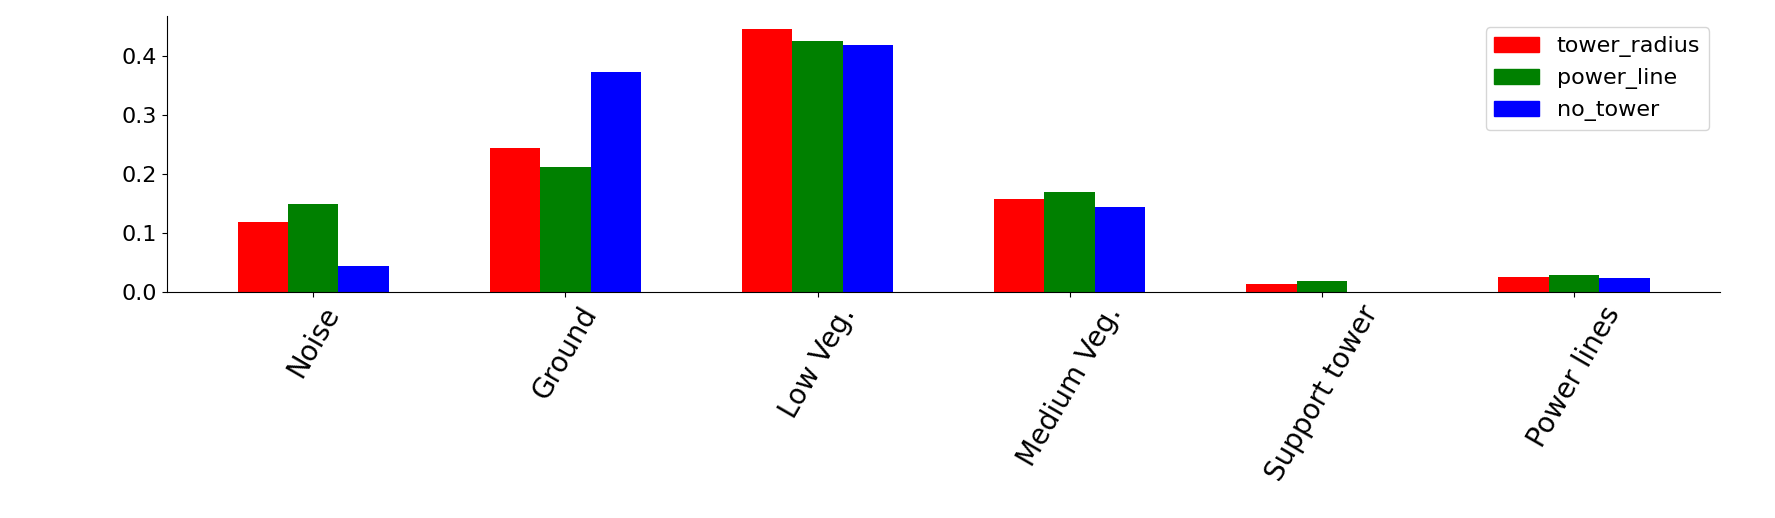
\includegraphics[width=\linewidth]{ts40k/Teaser/ts40k_class_densities.png}
                  \caption{Sample type density}
                  \label{fig:density1}
            \end{subfigure}
            \hfill
            \begin{subfigure}[b]{1.0\textwidth}
                  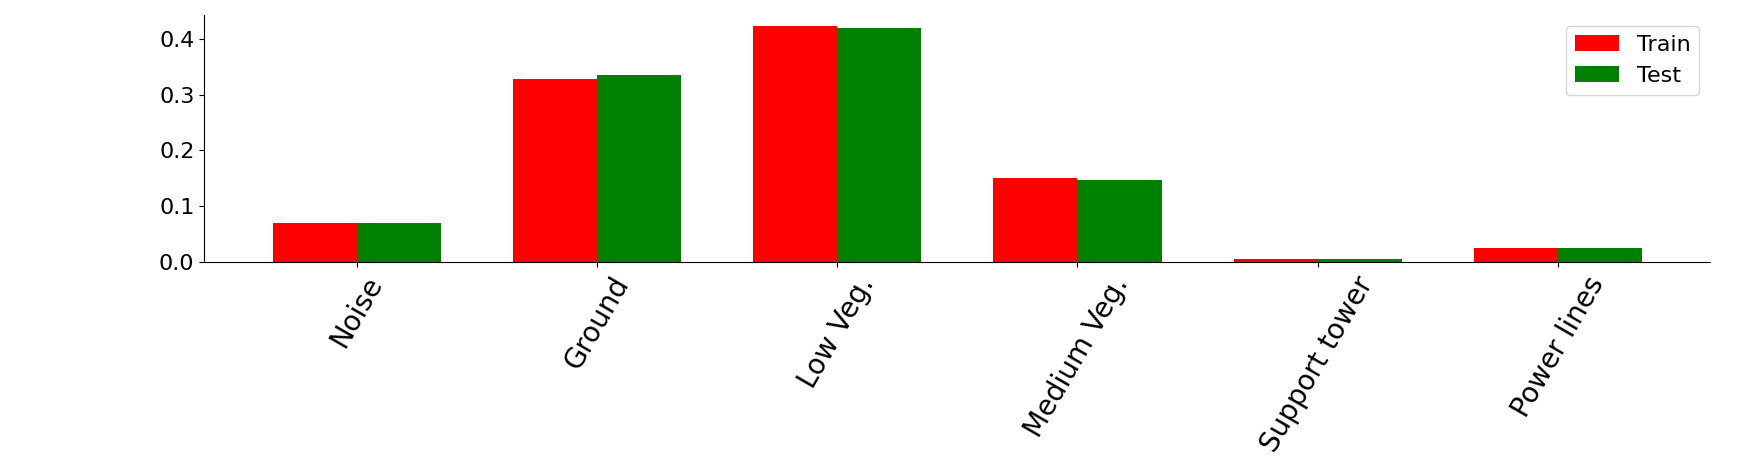
\includegraphics[width=\linewidth]{ts40k/Teaser/ts40k_train_test_distribution.png}
                  \caption{Overall train/test class density}
                  \label{fig:density2}
            \end{subfigure}
      \end{minipage}

      \caption[TS40K dataset overview]{The TS40K dataset is derived from raw 3D scans illustrated in Figure~\ref{fig:teaser-raw-sample} and processed into three different sample types: \textit{(1) Tower-radius} focuses on the towers that support power lines and its environment (Fig.~\ref{fig:teaser-tower-radius}). \textit{(2) Power-line} samples have power lines as their main focus in the 3D scenes (Fig.~\ref{fig:teaser-power-line}). \textit{(3) No-tower} samples represent rural terrain where the transmission system is located, excluding supporting towers but potentially including power lines (Fig.~\ref{fig:teaser-no-ts}).
            %
            In Figures~\ref{fig:density1} and~\ref{fig:density2}, we showcase the semantic
            class densities of the TS40K dataset. Figure~\ref{fig:density1} illustrates the
            class density for each of the sample types and Figure~\ref{fig:density2} shows
            the overall class density in the TS40K train and test sets.} \label{fig:teaser}
\end{figure}

\subsection{Problem Statement and Motivation}

Routine inspection of transmission infrastructure is a critical task for
ensuring grid reliability and public safety. Traditional inspection methods,
while effective at small scales, face increasing challenges as transmission
networks grow larger and more geographically dispersed. The integration of
UAV-mounted LiDAR sensors has improved data collection efficiency, enabling the
acquisition of dense 3D point clouds of transmission corridors. However, as
discussed in Section~\ref{sec:3d_scene_understanding_power_grid}, the
downstream analysis of this data remains heavily reliant on manual
interpretation, leading to operational bottlenecks, high costs, and elevated
risk of human error.
%
Machine learning methods, particularly 3D semantic segmentation and object
detection, have shown promise in automating parts of this workflow. Yet
existing 3D datasets, predominantly focused on urban driving or indoor
environments, fail to capture the unique challenges of rural transmission
systems. Moreover, the risk tolerance in this domain is considerably lower:
false negatives can lead to undetected faults or vegetation risks, while false
positives impose unnecessary operational costs.

Addressing these gaps requires not only advances in model development, but also
the creation of domain-specific datasets that accurately reflect the
operational complexity and safety-critical nature of power grid inspection
tasks.
%
Additionally, the need for automation in this domain is not purely about
efficiency, it is driven by operational risk and cost. False negatives can have
severe consequences, while false positives can waste critical resources. Thus,
any proposed system must prioritize recall without sacrificing robustness or
operational viability.

\subsection{Methodology}

The TS40K dataset~\cite{Lavado_2025_WACV} was developed to serve as a realistic
benchmark for 3D scene understanding in the context of rural power grid
inspections. The dataset captures over 40,000 kilometers of electrical
transmission systems using UAV-mounted LiDAR, resulting in high-density point
clouds with minimal occlusion and high spatial precision.

Several design considerations were prioritized during dataset creation
%
\begin{enumerate}
      \item \textbf{Operational Realism:}
            The dataset was curated from real-world inspection missions conducted by
            EDP NEW and Labelec in past years. Annotations were produced by maintenance
            personnel with a focus on inspection, not machine learning
            optimization.
            As a result, the dataset includes noisy labels and class ambiguities.
            To still allow for ML model training, we introduce a mapping from inpection
            annotations to semantically meaningful classes. The semantic classes were defined
            in collaboration with field experts to highlight elements critical for risk
            assessment, including different types of vegetation, power lines,
            and support towers.
            The labelling inconsistencies serve as a valuable resource for
            evaluating the robustness of machine learning models in real-world
            conditions.
            %
      \item \textbf{Sensor and Annotation Noise:}
            TS40K preserves sensor artifacts (e.g., spurious points from weather interference)
            and manual annotation inconsistencies, which are common in operational scans but
            typically absent from academic datasets.
            %
      \item \textbf{Structural Imbalance:}
            To mirror real-world distributions,
            no artificial oversampling of infrastructure elements was performed.
            Power lines and towers comprise less than 2\% of the total point count,
            creating a challenging but authentic class imbalance for model training.
            %
      \item \textbf{Safety Partitioning:}
            The original LiDAR scans consist of long landstrips that follow the
            power grid infrastructure. In order to safeguard the network's topology,
            the dataset is partitioned into three non-contiguous distinct sample types:
            tower-radius, which encompasses a radius of 50 meters around a single tower;
            power-line, which includes two consecutive towers and the power line between them;
            and no-tower samples, consisting of segments with no support towers to maintain
            the original data distribution.
            %
            Additionally, the georeference annotations are removed and the spatial
            coordinates in each sample are normalized between 0 and 1.
            %
            These measures are essential to enable the public access of the dataset while
            ensuring the safety of the power grid infrastructure.

\end{enumerate}

\subsection{Results}

Benchmarking state-of-the-art 3D semantic segmentation models on TS40K
highlights the substantial challenges inherent to power grid inspection tasks.
Several baselines were evaluated, including PointNet~\cite{qi2017pointnet},
PointNet++\cite{qi2017pointnet++}, KPConv\cite{thomas2019kpconv},
RandLaNet~\cite{hu2020randla}, and the Point Transformer
family~\cite{zhao2021point}.
%
Overall, Point Transformer V2 and V3 models consistently outperformed other
architectures. Under the best experimental settings (weighted loss, noise class
modeling, ground point removal), Point Transformer V3 achieved an mIoU of
67.46\% and Intersection over Union scores of 65.05\% for towers and 96.25\%
for power lines.
%
3D object detection experiments exhibited similar trends. Using detectors such as
PV-RCNN~\cite{shi2020pv}, Part-A2 Net~\cite{shi2020points}, and
PointRCNN~\cite{shi2019pointrcnn}, the best models achieved mean Average Precision
(mAP) scores around 60\%, with power lines being detected more reliably than support
structures or medium vegetation. These results reaffirm the difficulty of detecting
small, cluttered, and partially occluded objects in rural transmission environments.

The application of 3D semantic segmentation models to TS40K demonstrates that
transformer-based architectures are capable of accurately identifying major
infrastructure components, particularly power lines, even under conditions of
moderate noise and structural variability.
%
Supporting towers remain more challenging to segment, particularly in the
presence of occlusions or non-standard infrastructure.
%
Building on these findings, we successfully designed a cost-aware decision
support system for power grid inspection, with model optimization explicitly
aligned with operational risk priorities. By adopting the F2 score as the
primary evaluation metric, the system emphasizes recall over precision,
ensuring that potential faults or vegetation risks are more likely to be
detected, even at the expense of a higher false positive rate. Under this
formulation, the Point Transformer V3 model achieved F2 scores of 96.05\% for
power lines and 87.37\% for towers, demonstrating its suitability for
integration into inspection workflows where missing critical faults carries
substantial operational consequences.

\section{Building GENEOs for Power Grid Inspection}\label{sec:scenenetv1}

\begin{figure}[ht]\label{fig:gnet_overview}
      \centering
      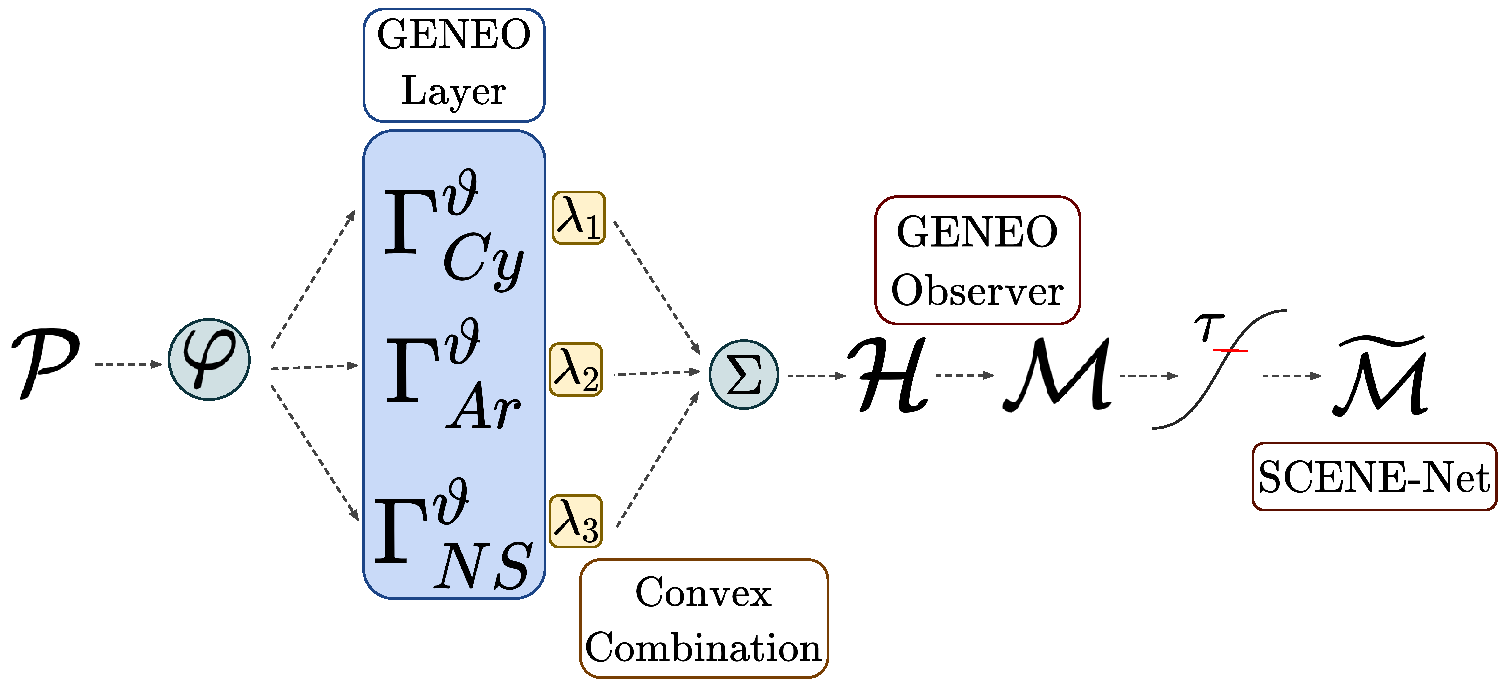
\includegraphics[width=.9\columnwidth]{scenenet/GNet_Overview.pdf}
      \caption[SCENE-Net Architecture]{Pipeline of SCENE-Net: an input point cloud  $\mathcal{P}$ is measured according to function $\varphi$ and voxelized. This representation then is fed to a GENEO-layer, where each operator $\Gamma_i^{\vartheta_i}$ separately convolves the input.
            A GENEO observer $\mathcal{H}$ is then achieved by a convex combination of the operators in the GENEO layer.
            $\mathcal{M}$ transforms the analysis of the observer into a probability of belonging to a tower. %
            Lastly, a threshold operation is applied to classify the voxels. Note that this final step occurs after training is completed.
      }
\end{figure}
\subsection{Problem Statement and Motivation}
As discussed in Section~\ref{sec:3d_scene_understanding_power_grid}, power grid
inspection tasks demand machine learning models that are both operationally
reliable and intrinsically interpretable. Black-box deep learning models, while
achieving high accuracy on academic benchmarks, provide limited insight into
their decision-making processes, which is unsuitable for deployment in
safety-critical settings.
%
The TS40K dataset adds to these challenges by introducing real-world
imperfections such as annotation noise and class imbalance. In this setting,
our goal is to design models whose internal representations are intrinsically
meaningful and explainable, while also achieving a good performance on semantic
segmentation tasks.

We take the first step to accomplish this with the adoption of SCENE-Net, a 3D
semantic segmentation model based on the Group Equivariant Non-Expansive
Operators (GENEOs).
%
SCENE-Net was originally developed during previous MSc
research~\cite{lavado2022detection}, targeting the detection of pole-like
structures in 3D point clouds through interpretable geometric observers. In the
present work, we extend SCENE-Net by incorporating additional GENEOs and by
evaluating its performance on external benchmarks.

\subsection{Methodology}

SCENE-Net instantiates the GENEO framework presented in
Section~\ref{sec:geneos} within the context of rural power grid inspection. The
model represents 3D point clouds through a perception pair $(\Phi, G)$, where
$\Phi$ denotes the space of admissible observations and $G$ encodes geometric
transformations such as translations and rotations.
%
Specifically, we define $\varphi \in \Phi$ as an occupancy grid, which
represents a point cloud as a voxel grid where each voxel is assigned a binary
value indicating the presence or absence of points.
%
In turn, $G$ encompasses three geometric priors tailored for pole detection:
\begin{itemize}
      \item \textbf{Cylinder GENEO:}
            Designed to detect vertical, cylindrical structures corresponding
            to the main body of towers and poles. The operator parameters include
            the radius and height of the cylinder.
            %
      \item \textbf{Arrow GENEO:}
            Introduced to model the conical intersections where towers connect
            with power lines. It is parameterized by height, base radius,
            and apex angle.
            %
      \item \textbf{Negative Sphere GENEO:}
            Acts to suppress clutter from spherical structures such as vegetation.
            This operator has parameters corresponding to sphere radius and
            negative score.
\end{itemize}

Each GENEO is built on top of the convolution operator with carefully designed
kernels, thus offering both a computationally efficient operation and
equivariance with respect to translations.
%
During training, it is not the kernels themselves that are fine-tuned with
back-propagation, since this would not preserve equivariance at each
optimization step. Instead, the error is propagated to the shape parameters of
each operator.
%
Moreover, each operator produces an intermediate feature map highlighting
regions of the input point cloud (now voxelized) that conform to the
corresponding geometric pattern.

Subsequently, the GENEO outputs are combined via a convex combination. Let
$\psi_i(x)$ denote the output of the $i$-th GENEO at location $x$, and
$\lambda_i \geq 0$ its convex coefficients. The combined output is:

\begin{equation}
      \gamma(x) = \sum_{i=1} \lambda_i \psi_i(x) \quad \text{s.t.} \quad \lambda_i \geq 0, \quad \sum_{i=1} \lambda_i = 1.
\end{equation}
%
This way, we ensure the the resulting observer $\gamma$ remains within the
space of GENEOs, thus preserving both group equivariance w.r.t. $G$ and
non-expansivity. The convex coefficients $\lambda_i$ represent the overall
contribution of each operator to the observer analysis. The parameters of each
GENEO and $\lambda_i$ grant our model its intrinsic interpretability.

The combined observer output is passed through a non-linear mapping to produce
a final probability score for the presence of pole-like structures for each
voxel:

\begin{equation}
      m(x) = {\left(\tanh(\gamma(x))\right)}_+,
\end{equation}

where ${(\cdot)}_+$ denotes the ReLU activation function.
%
Negative signals in $\gamma(x)$ represent patterns that do not exhibit the
desired geometric properties. Conversely, positive values quantify their
presence. Therefore, $\tanh$ compresses the observer’s value distribution into
$[-1, 1]$, and the ReLU is then applied to enforce a zero probability for
negative signals. Lastly, a probability threshold $\tau \in [0, 1]$ is defined
through hyperparameter fine-tuning and applied to $m(x)$.

\subsection{Results}

The evaluation of SCENE-Net focused on three research axes: parameter
interpretability, parameter efficiency, and segmentation performance.

\textbf{Parameter Interpretability.} \;
To assess the interpretability of SCENE-Net, we inspected its eleven trainable
parameters after training.
%
Each GENEO is parameterized by a set of shape parameters $\vartheta_i$ (e.g.,
height, radius, and apex angle), which are learned during training.
%
In addition, the model includes a set of convex coefficients $\lambda_i$ that
determine the contribution of each GENEO to the final output.
%
Globally, the Negative Sphere dominated SCENE-Net's decision-making, accounting
for 76.34\% of the model’s weight. The Arrow contributed 16.16\%, while the
Cylinder accounted for 7.50\%.
%
At a local, post hoc level, SCENE-Net enables tracing individual predictions
back to specific GENEO contributions. For instance, correct detections of
supporting towers were predominantly influenced by the Arrow operator, with the
Cylinder operator aiding in reducing false positives from surrounding
vegetation. The Negative Sphere acted as a stabilizer, balancing the
contributions of structural detectors and maintaining robustness against
background noise.

\textbf{Parameter Efficiency.} \;
SCENE-Net uses only eleven trainable parameters to perform 3D semantic
segmentation, compared to the millions of parameters typically employed by
standard point cloud segmentation models. This extreme parameter efficiency
serves as a proof of concept for the viability of GENEO-based inductive biases:
by embedding geometric priors directly into the model architecture, it is
possible to achieve meaningful scene understanding with minimal learnable
complexity. This efficiency also contributes to improved generalization and
robustness across datasets.

\textbf{Segmentation Performance.} \;
On the TS40K dataset, SCENE-Net achieved a 38\% increase in Precision and a 5\%
increase in Intersection over Union (IoU) relative to a baseline CNN of similar
depth, but showed a 13\% decrease in Recall.
%
Additionally, evaluation on SemanticKITTI showed that SCENE-Net achieved a pole
class IoU of 57.5\%, confirming its ability to generalize pole-like structure
detection beyond the specific characteristics of the TS40K domain.

% \section{Stochastic Augmented Lagrangian for Dynamic Regularization}\label{sec:SAL}

% \subsection{Problem Statement and Motivation}

% \subsection{Methodology}

% \subsection{Results}

\section{Geometric Inductive Biases as Feature Extractors for 3D Scene Understanding}\label{scenenetv2}

\begin{figure}[ht]
      \centering
      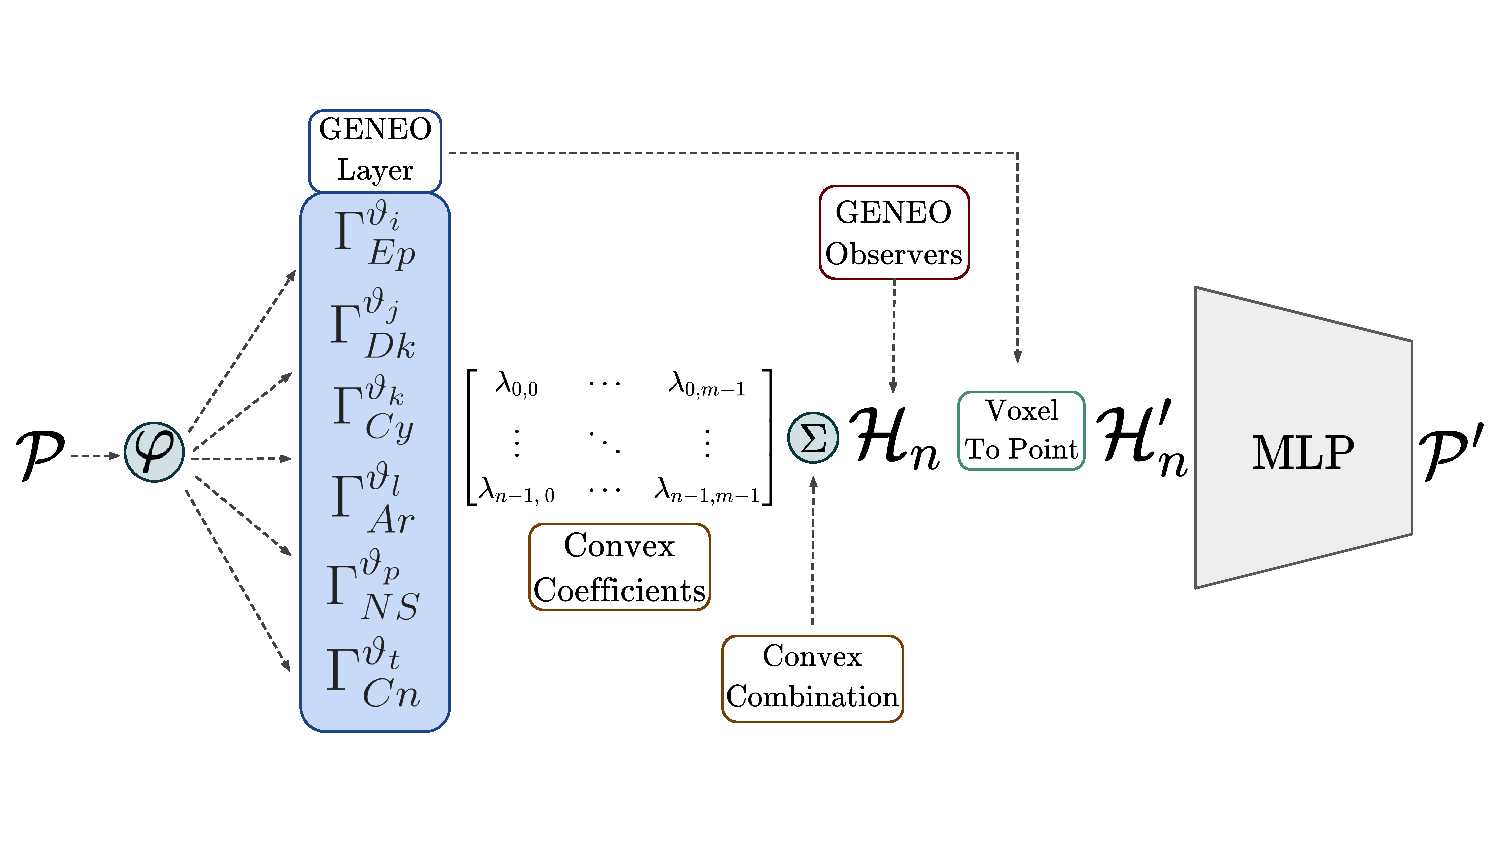
\includegraphics[width=1.0\columnwidth]{scenenetv2/SCENE-NETV2.pdf}
      \caption[SCENE-Net v2 Architecture]{SCENE-Net v2 architecture: An input point cloud $\mathcal{P}$ is initially measured according to function $\varphi$ and discretized into a 3D voxel grid. A GENEO Layer with $m$ GENEO kernels then extracts geometric information from the voxel grid. Each operator $\Gamma$ is based on the convolution operation and is derived from six parametric families of geometric shape priors. Following this, $n$ GENEO observers $\mathcal{H}$ are obtained through a convex combination of the GENEO Layer outputs, with the convex coefficients illustrated by $\lambda$. These observers learn to combine features extracted in the GENEO Layer, recognizing complex geometric patterns in the data. Finally, the shape prior features from the GENEO Layer and the GENEO observers are merged via a voxel-to-point transformation, resulting in $\mathcal{H}'$, which is then classified using a Multi-Layer Perceptron (MLP).
      }
      \label{fig:gnet_overview}
\end{figure}

\subsection{Problem Statement and Motivation}

SCENE-Net demonstrated that geometric priors encoded via GENEOs could be used
to detect pole-like structures in 3D point clouds with strong interpretability
and extreme parameter efficiency. However, its application is limited: the
model is specialized for binary segmentation and incapable of handling the
complexity of multiclass 3D scene understanding. Additionally, while using only
eleven trainable parameters served as a compelling proof of concept, this
design lacks the flexibility needed for broader semantic tasks.
%
To enable multiclass segmentation while preserving the benefits of structured
geometric reasoning, we introduce SCENE-Net v2. This new formulation uses
GENEOs not as end-to-end predictors, but as interpretable feature extractors
within a larger pipeline that includes a black-box classifier. The resulting
architecture is a grey-box model: its initial layers retain full
interpretability, while its classification stage leverages the capacity
black-box network (e.g., MLPs) to learn complex decision boundaries.
%
This represents a shift in paradigm. Rather than viewing geometric inductive
biases as capable of solely performing segmentations, we now treat them as
meaningful, task-aligned representations that can support more expressive
classifiers. SCENE-Net v2 implements this approach and evaluates its
effectiveness in multiclass 3D segmentation.

\subsection{Methodology}

SCENE-Net v2 also builds upon the GENEO formalism (Section~\ref{sec:geneos})
and introduces a systematic process for multiclass 3D segmentation with strong
geometric inductive biases.
%
Firstly, Input point clouds are voxelized and transformed into binary occupancy
functions, forming the basis for functional observers.
%
Unlike SCENE-Net v1, which used a single observer composed of one instance of
each GENEO, SCENE-Net v2 scales up to multiple instances per GENEO type,
enabling greater representational diversity while maintaining computational
efficiency. The model employs six GENEO types:
\begin{itemize}
      \item \textbf{Cylinder}: Detects vertical cylindrical structures.
      \item \textbf{Arrow}: Captures conical intersections and vertical connections.
      \item \textbf{Negative Sphere}: Suppresses spherical clutter like vegetation.
      \item \textbf{Disk}: Detects planar surfaces with rotational flexibility.
      \item \textbf{Cone}: Captures narrow conical shapes like small tree tops.
      \item \textbf{Ellipsoid}: Generalizes spheres to model elongated or compressed structures.
\end{itemize}
%
Then, GENEO outputs are combined into $n$ observers $\gamma_i$ via a convex
combination:

\begin{equation}
      \gamma_i(x) = \sum_{j=1}^m \Lambda_{ij} \psi_j(x) \quad \text{s.t.} \quad \Lambda_{ij} \geq 0, \quad \sum_{j=1}^m \Lambda_{ij} = 1,
\end{equation}

where $\Lambda_{ij}$ is the convex coefficient for the $j$-th GENEO in the
$i$-th observer. This preserves equivariance and non-expansivity.
%
Lastly, the outputs of the GENEO layer and constructed observers are converted
from voxel grids back to point-level features. These are passed into a
lightweight Multi-Layer Perceptron (MLP), which acts as a black-box classifier
to assign semantic labels. This separation of interpretable feature extraction
and expressive classification constitutes a grey-box architecture, balancing
explainability with capacity.

\subsection{Results}

In the evaluation of SCENE-Net v2, we focus on the same three axes: parameter
interpretability, parameter efficiency, and segmentation performance.

\textbf{Parameter Interpretability.} \;
While the inclusion of a black-box classifier reduces overall transparency
relative to SCENE-Net, the GENEO layer remains fully interpretable. Each
GENEO instance is defined by explicit geometric parameters, and each observer's
contribution is governed by convex weights. Post-training, it is possible to
analyze individual predictions by tracing them back through the GENEO
activations, providing insights into which geometric patterns are driving each
classification. This post hoc traceability offers a valuable middle ground:
although not a pure white-box model, SCENE-Net v2 allows practitioners to
inspect and reason about the internal mechanisms of specific predictions.

\textbf{Parameter Efficiency.} \;
SCENE-Net v2 retains a highly compact design. The full model uses approximately
240K parameters, which is orders of magnitude smaller than conventional
segmentation networks like Point Transformer V2 (46M). Only 540 parameters are
used in the GENEO feature extraction layer. This efficient use of parameters
validates the GENEO framework as a lightweight but expressive representation
for 3D scene understanding and supports deployment in resource-constrained
environments.

\textbf{Segmentation Performance.} \;
On the TS40K dataset, SCENE-Net v2 achieves a mean Intersection over Union
(mIoU) of 45.54\%, outperforming traditional baselines such as PointNet and
simple CNNs. When the GENEO features are combined with a the
CNN baseline, performance rises to 50.21\% mIoU. These results suggest that
geometric priors encoded via GENEOs can complement the flexibility of black-box
classifiers, leading to improved accuracy while preserving interpretability at
the feature level.
%
Ablation studies confirm that removing specific GENEO types degrades
performance, particularly the Cylinder GENEO, which plays a key role in
detecting towers and poles. This highlights the contribution of structured
geometric reasoning, even in a grey-box context.
%
Taken together, these results demonstrate that SCENE-Net v2 strikes a practical
balance between interpretability and performance. By repositioning geometric
inductive biases as feature extractors, our model offers a scalable and
explainable path forward for 3D semantic segmentation.

\section{Geometric Inductive Bias Library for Efficient 3D Scene Understanding (GIBLi)}\label{sec:gibli}

\begin{figure}[ht]
      \centering
      \begin{subfigure}[t]{0.48\columnwidth}
          \centering
          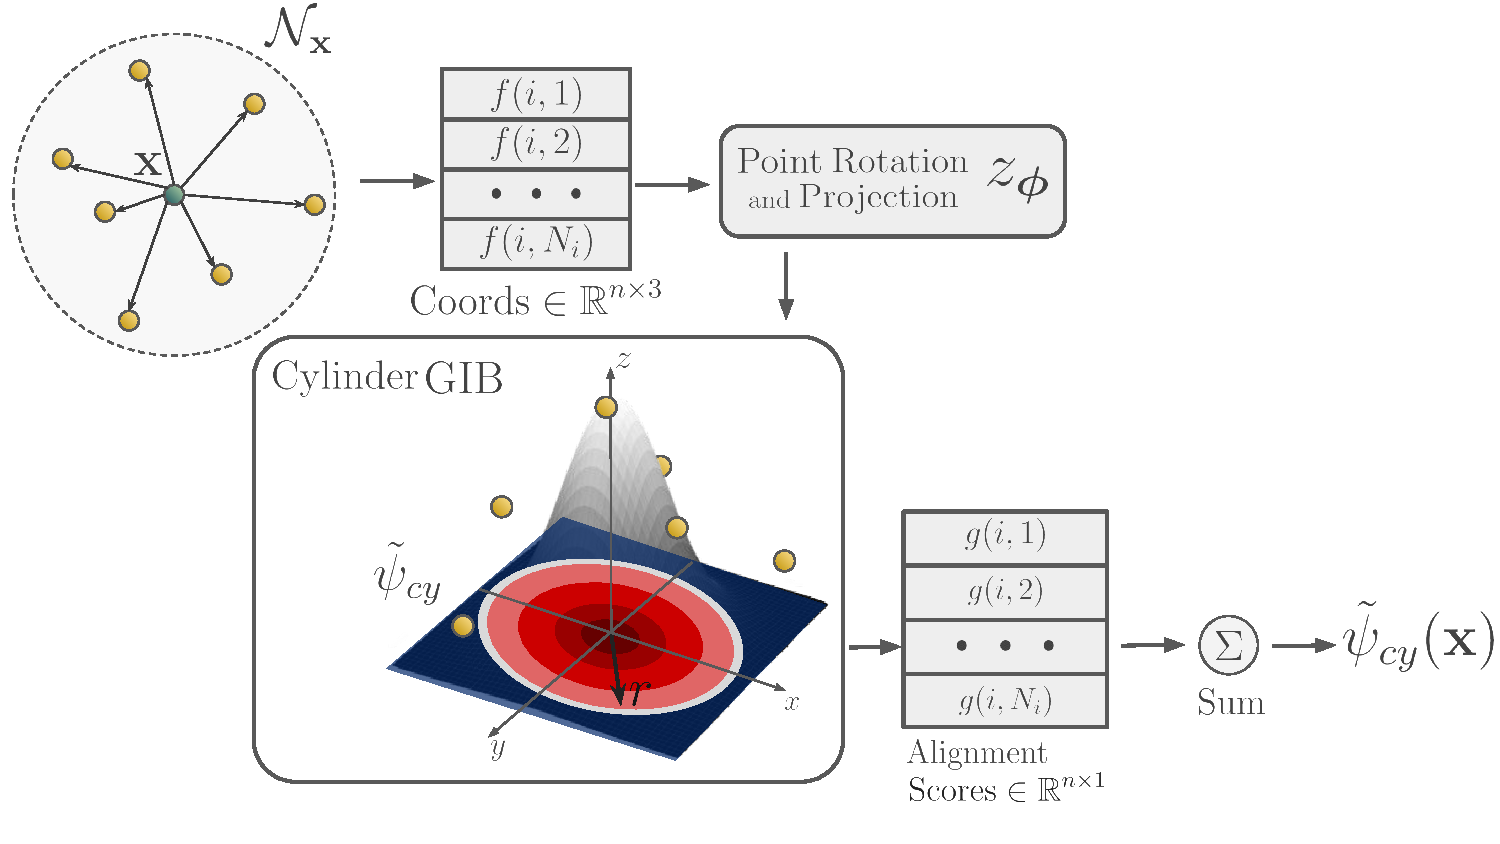
\includegraphics[width=\linewidth]{gibli/ICCV_GIBLi_Cy_GIB.pdf}
          \caption{Illustration of the Cylinder geometric inductive bias (GIB) applied to a local neighborhood.}
          \label{fig:gib_cy}
      \end{subfigure}
      \hfill
      \begin{subfigure}[t]{0.48\columnwidth}
          \centering
          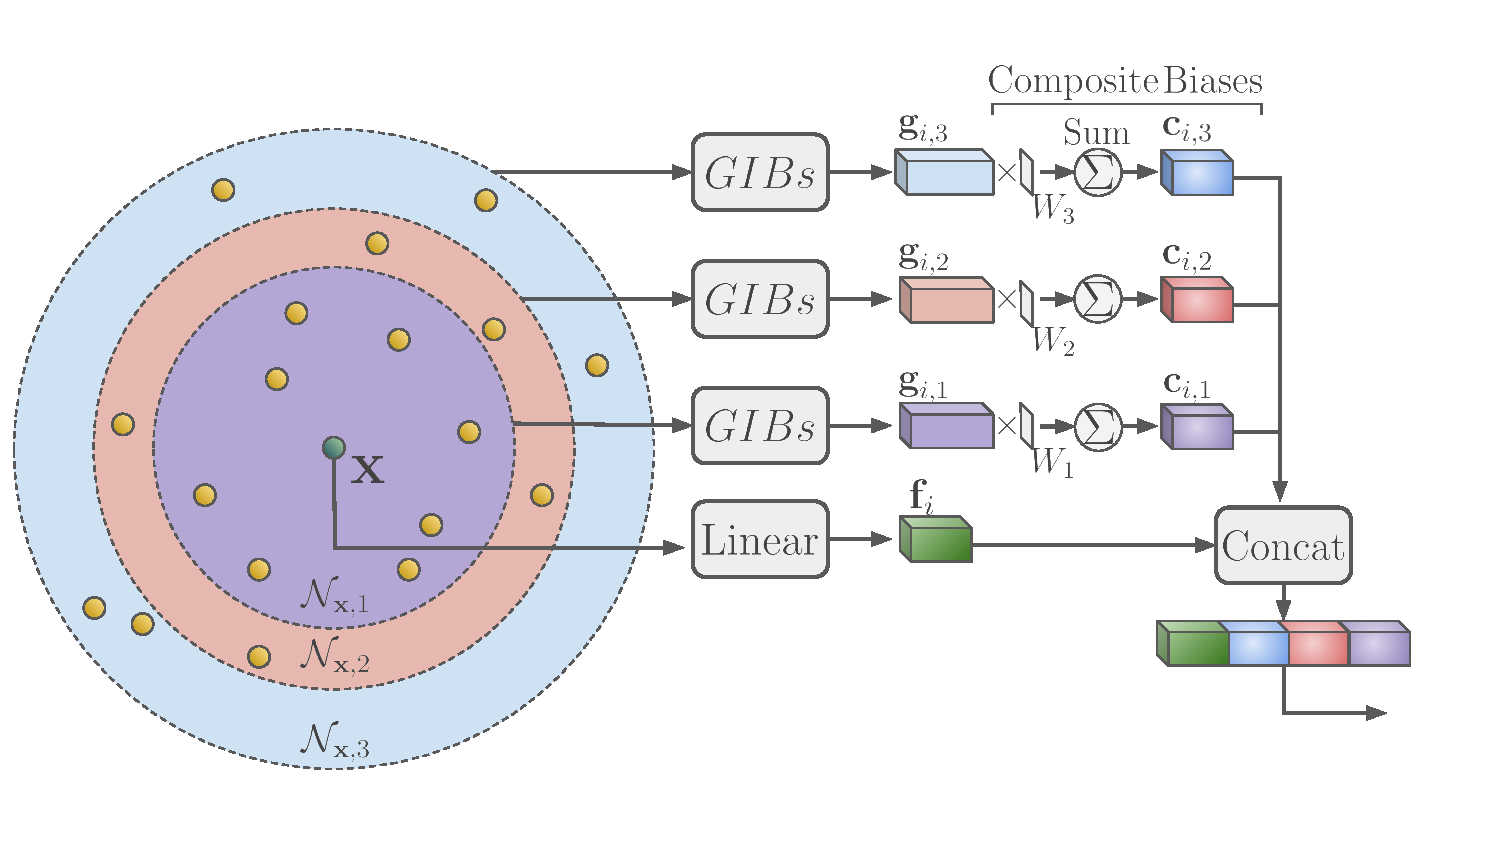
\includegraphics[width=\linewidth]{gibli/ICCV_GIBLi_GIBLiLayer.pdf}
          \caption{Illustration of the GIBLi-Layer.}
          \label{fig:gibli-layer}
      \end{subfigure}
      \caption[GIBLi Overview]{(Left) Cylinder GIB computing alignment scores. (Right) GIBLi-Layer extracting geometric features from a local neighborhood.}
      \label{fig:gib_pair}
  \end{figure}

\subsection{Problem Statement and Motivation}

While SCENE-Net v2 demonstrated that geometric inductive biases (GIBs) can
enhance 3D scene understanding by acting as interpretable feature extractors,
it also revealed important limitations. Most critical is the reliance on
voxelization: mapping irregular point clouds onto structured grids incurs a
heavy memory footprint and computational cost. This approach is not compatible
with large-scale point clouds and limits scalability.
%
Moreover, with the paradigm shift to treating GIBs as feature extractors rather
than full predictors, it became clear that a mismatch remained: most
state-of-the-art (SOTA) 3D learning architectures operate directly on raw point
clouds. To fully integrate geometric priors into modern pipelines, GIBs must
also act directly in the point cloud domain.
%
We propose a new framework, GIBLi, to address these limitations. It extends
geometric inductive biases to raw point clouds by treating them as geometric
graphs, enabling modular and scalable integration with any backbone
architecture. By providing structured geometric information at the feature
level, GIBLi aims to accelerate convergence, improve robustness, and reduce the
burden on black-box models, which otherwise must learn geometric structure
purely from data.

Thus, this work represents a further evolution of the SCENE-Net line: moving
from voxelized feature extraction to point-based, fully modular, and scalable
geometric reasoning, with the goal of achieving better alignment with SOTA
pipelines while preserving interpretability in feature extraction.

\subsection{Current Methodology}

The goal of GIBLi is to develop a modular GIBLi-Layer that can be inserted into
any point-based network architecture. The GIBLi-Layer operates as follows:

Input point clouds are interpreted as geometric graphs, with local
neighborhoods defined through $k$-nearest neighbors or radius-based queries. To
capture structures at multiple scales, our GIBLi-Layer considers multiple
neighborhoods per point, operating with varying radius or $k$ values.
%
For each neighborhood, multiple geometric inductive biases (GIBs) are applied.
Each GIB is a structured parametric function $\psi(x; \vartheta, R)$, where
$\vartheta$ are shape parameters and $R \in SO(3)$ is a learnable rotation
matrix, allowing the GIB to align with local data orientation.
%
The GIB library includes: cylinders, cones, disks, and ellipsoids.

For each kernel type, both \textbf{solid} and \textbf{hollowed} versions are
defined. Hollowed variants increase the flexibility of the geometric matching,
allowing the model to represent structures with internal voids or shells, such
as thin poles or tree canopies.

Each GIB produces a feature vector for each point, encoding how strongly the
local neighborhood conforms to the geometric pattern. The outputs of all GIBs
across all neighborhood scales are concatenated with the existing features of
each point, forming an enriched representation.
%
This enriched feature tensor is then passed to downstream modules (e.g., SOTA
backbones) for further processing. Thus, GIBLi provides a grey-box feature
extraction stage that enhances SOTA models without disrupting their core
architectures.

\subsection{Challenges and Current Progress}

Despite the promising design of GIBLi, several technical and conceptual
challenges arise from adapting geometric inductive biases to operate directly
on point clouds. Here, we outline the main challenges encountered so far and
the current progress toward addressing them:

\textbf{Efficient Implementation on Point Clouds.} \;
Developing GIBLi requires non-trivial extensions to standard point cloud processing.
Unlike grid-based convolutions, there are currently no native operations in
mainstream machine learning libraries (e.g., PyTorch, TensorFlow) that support
GIB-based operations over local geometric graphs. This demands custom operator
design to achieve acceptable efficiency at scale.

\textbf{Interpretability-Performance Trade-off.} \;
As backbone models grow in complexity, the overall interpretability of the
system diminishes compared to previous white-box designs.
Nonetheless, GIBLi preserves interpretability at the feature extraction stage:
each enriched feature vector can be traced back to specific GIB activations,
enabling post hoc analysis of how geometric priors contribute to individual predictions.

\textbf{Designing Effective and Flexible GIB Operators.} \;
Without the regular structure of voxel grids, defining efficient, expressive,
and differentiable geometric operators on irregular point clouds presents new
challenges.

Currently, our work focuses on refining the efficiency of GIBLi-Layers,
expanding the library of inductive biases, and evaluating their integration
into diverse SOTA architectures in several 3D benchmarks. A key research goal
is to assess whether GIBLi can systematically improve convergence, robustness,
and final accuracy in large-scale 3D semantic segmentation tasks.

% ------------------------------------
\section{Summary and Outlook}\label{sec:summary_outlook}

This research explores the use of geometric inductive biases (GIBs) as a
foundation for interpretable and efficient 3D scene understanding. Beginning
with SCENE-Net, we demonstrated that structured geometric priors could drive
pole-like structure detection with extreme parameter efficiency and intrinsic
interpretability. However, the specialization and limited scalability of
SCENE-Net motivated further research.
%
SCENE-Net v2 extended this approach to multiclass semantic segmentation,
introducing a grey-box architecture where geometric priors serve as feature
extractors for downstream black-box classifiers. This shift enabled a more
flexible and scalable integration of GIBs, though at the cost of some
transparency relative to the original design.
%
In parallel, we developed the TS40K benchmark, the first large-scale, publicly
available 3D dataset focused on rural power grid inspection. TS40K captures the
operational complexities of real-world transmission systems, including label
noise, structural variability, and severe class imbalance.
%
Building on these insights, GIBLi represents the next step: generalizing GIBs
to operate directly on raw point clouds without voxelization. By treating point
clouds as geometric graphs and equipping GIBs with learnable rotations and
hollowed variants, GIBLi aims to unify geometric reasoning with
state-of-the-art 3D learning practices. The goal is to provide structured,
interpretable features that accelerate convergence, improve robustness, and
enhance segmentation performance across large-scale benchmarks such as TS40K
and beyond.

Work is ongoing to refine the implementation of GIBLi, optimize its
computational efficiency, and systematically evaluate its integration into
modern architectures. This line of research aims to demonstrate that explicit
geometric priors can remain relevant and valuable even as 3D machine learning
continues to evolve toward increasingly data-driven regimes.